% !TEX root = main.tex

\section{彩色图像处理}
图像主要包括三方面内容:颜色、形状、纹理

\subsection{颜色特性}
彩色光的3个基本量:
\begin{itemize}
	\item 辐射率:从光源流出能量的总量,用Watt表示
	\item 光强:观察者从光源接受的能量总和,用流明表示
	\item 亮度:主观描绘子,人感觉到的
\end{itemize}

人眼中有600-700万个锥状体分别对红色(700nm)、绿色(546nm)、蓝色(435.8nm)敏感\footnote{注意这里只是人为定义波长,真正的红绿蓝是一段波长区间。}。
65\%对红光敏感、33\%对绿光敏感、2\%对蓝光敏感。

三基色原理:
红绿蓝为三种基色,组成RGB三维加性空间
\begin{figure}[H]
\centering
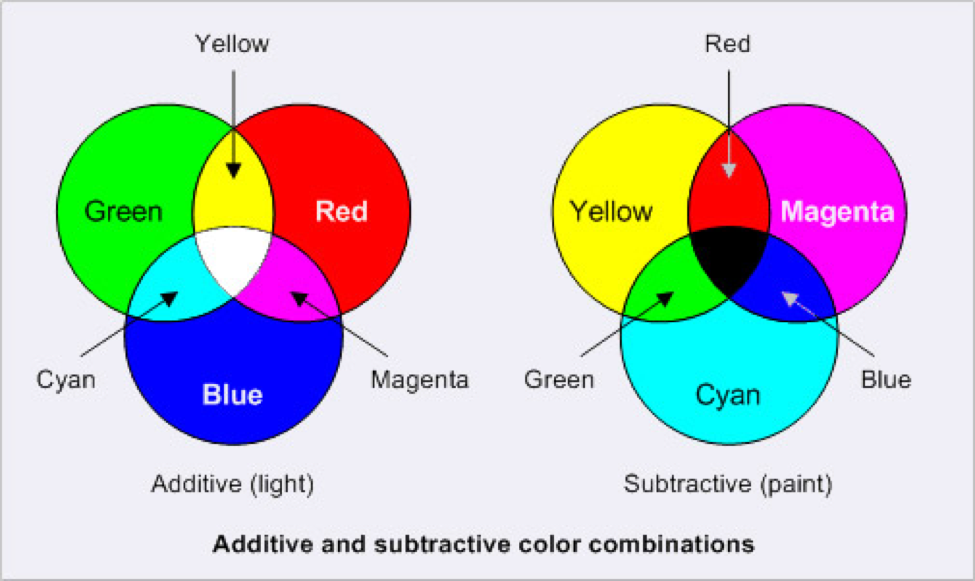
\includegraphics[width=0.8\linewidth]{fig/rgb_and_cmyk.png}
\end{figure}

区别颜色的特性:亮度、色调、色饱和度。
颜色通常用亮度和彩色表征,色调、和饱和度统称为彩色色度。
设$X,Y,Z$为红绿蓝的系数,则做归一化,得到颜色的唯一比例
\[\begin{aligned}
x&=\frac{X}{X+Y+Z}\\
x&+y+z=1
\end{aligned}\]

真彩色(24b):RGB各用一个字节表示,共216种安全色(各种设备都可以正常显示),剩下40个为控制字节

\subsection{颜色空间}
常见的颜色空间\footnote{\url{https://en.wikipedia.org/wiki/List_of_color_spaces_and_their_uses}}如下
\begin{itemize}
	\item RGB:\textbf{加性空间},与人眼视觉系统密切相连。
	\begin{itemize}
		\item RGBA:加上透明通道
		\item sRGB(standard):Microsoft
		\item Adobe RGB:打印出来更接近原色
	\end{itemize}
	\item CMY/CMYK:青色(cyan)、品红(magenta)、黄色(yellow)、黑色(key/black),主要用于\textbf{打印}。打印主要靠反射(\textbf{减性空间}),如黄色是白光将蓝色吸收掉。由于油墨很少能将颜色都吸收掉,深色效果较差,故加入一种黑色K。
	\item HIS/HSL/HSV:色度(hue)、亮度(intensity)、饱和度(saturation),亮度与色彩分离。广泛应用于计算机视觉、图像检索和视频检索。
	\item CIE:第一个基于人类视觉感知的颜色空间。CIE-XYZ(1931)是在RGB系统的基础上,用数学方法,选用三个理想的原色来代替实际的三原色,从而将CIE-RGB系统中的光谱三刺激值和色度坐标r、g、b均变为正值。
	\item Lab:Lab模式既不依赖光线,也不依赖于颜料,它是CIE组织确定的一个理论上包括了人眼可以看见的所有色彩的色彩模式。Lab模式弥补了RGB和CMYK两种色彩模式的不足。同RGB颜色空间相比,Lab是一种不常用的色彩空间。它是一种设备无关的颜色系统,也是一种基于生理特征的颜色系统。
	这也就意味着,它是用数字化的方法来描述人的视觉感应。Lab颜色空间中的L分量用于表示像素的亮度,取值范围是$[0,100]$,表示从纯黑到纯白;a表示从红色到绿色的范围,取值范围是$[127,-128]$;b表示从黄色到蓝色的范围,取值范围是$[127,-128]$。
	\item YUV:明亮度(Y, Luminance/Luma)即灰阶值、色度(U/V, Chrominance/Chroma)用于指定像素颜色。包括YCbCr、YPbPr、YUV、Y'UV等,后两者通常用来编码电视的模拟信号\footnote{Y'UV的发明是由于彩色电视与黑白电视的过渡时期。黑白视频只有Y(Luma/Luminance)视频,也就是灰阶值。到了彩色电视规格的制定,是以YUV/YIQ的格式来处理彩色电视图像,把UV视作表示彩度的C(Chrominance或Chroma),如果忽略C信号,那么剩下的Y(Luma)信号就跟之前的黑白电视频号相同,这样一来便解决彩色电视机与黑白电视机的兼容问题。Y'UV最大的优点在于只需占用极少的带宽。},YCbCr用来描述数字的视频信号,适合视频与图片压缩以及传输,例如MPEG、JPEG。
\end{itemize}

关于不同颜色空间的优缺点可见\footnote{\url{https://blog.csdn.net/JiangHui1211/article/details/84592774}}。

\subsection{伪彩色处理}
根据一定的准则对灰度值赋以彩色的处理。
之所以需要伪彩色,是因为人类可以辨别上千种颜色和强度,但只能辨别二十几种\textbf{灰度}。
比如将不同灰度赋予不同颜色,得到热度图(heatmap)。

\subsection{全彩色处理}
两种处理方式:分通道处理、向量处理。

补色:两种颜色混在一起为白色(RGB补色为CMY)
\begin{figure}[H]
\centering
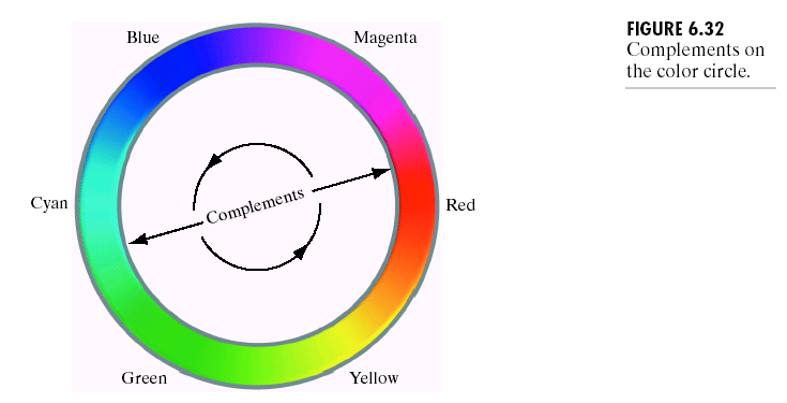
\includegraphics[width=0.6\linewidth]{fig/complements.png}
\end{figure}

\subsection{彩色分割}
\begin{itemize}
	\item HSI颜色空间分割直观,H色调图像方便描述彩色,S饱和度图像做模板分离感兴趣的特征区,I强度图像不携带彩色信息。如用门限产生二值图像,大于门限的像素赋为1,其他赋为0。
	\item RGB彩色空间直接,用欧式距离度量。
\end{itemize}
% 彩色空间的人脸检测

如果直接采用3个独立平面形成的合成梯度图可能导致彩色边缘检测错误,因此要采用Di Zenzo提出的方法。